\setlength{\columnsep}{3pt}
\begin{flushleft}
\bigskip

\paragraph{nmcli command}

\begin{itemize}
	\item nmcli stands for \textbf{network manager command line}.
	\item It is a command-line tool for controlling NetworkManager.
	\item Options with \textbf{nmcli} command:
	\begin{itemize}
		\item Display all available LAN card devices:
		\begin{tcolorbox}[breakable,notitle,boxrule=-0pt,colback=pink,colframe=pink]
			\color{black}
			\fontdimen2\font=1em
			Syntax: nmcli device show
			\newline
			or
			\newline
			Syntax: nmcli dev show
			\fontdimen2\font=4pt
		\end{tcolorbox}
		Eg:
		\begin{figure}[h!]
			\centering
			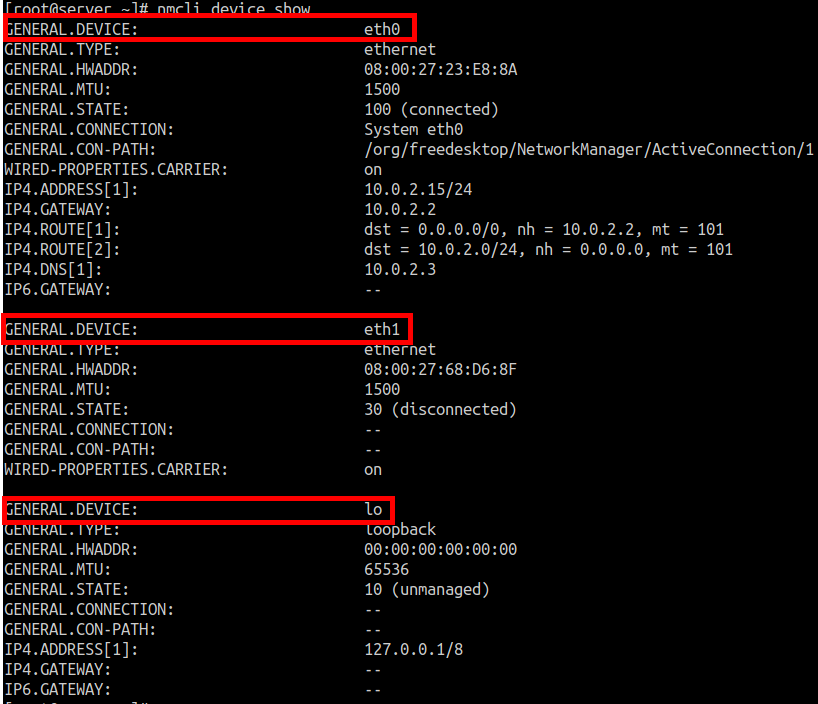
\includegraphics[scale=.35]{content/chapter14/images/cards.png}
			\caption{List of available devices}
			\label{fig:devices}
		\end{figure}		
		\newpage
		\item Display all available connections
		\begin{tcolorbox}[breakable,notitle,boxrule=-0pt,colback=pink,colframe=pink]
			\color{black}
			\fontdimen2\font=1em
			Syntax: nmcli connection show
			\newline
			or
			\newline
			Syntax: nmcli con show
			\fontdimen2\font=4pt
		\end{tcolorbox}
		Eg:
		\begin{figure}[h!]
			\centering
			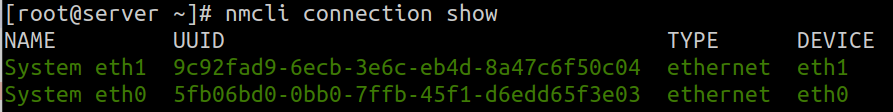
\includegraphics[scale=.35]{content/chapter14/images/show.png}
			\caption{List of available interfaces}
			\label{fig:list}
		\end{figure}		
	
		\bigskip
		\bigskip
		\item Add new connection to an interface:
		\begin{tcolorbox}[breakable,notitle,boxrule=-0pt,colback=pink,colframe=pink]
			\color{black}
			\fontdimen2\font=1em
			Syntax: nmcli connection add con-name <connection\_name> ifname <interface\_name> type ethernet
			\fontdimen2\font=4pt
		\end{tcolorbox}

		Eg:	
		\begin{tcolorbox}[breakable,notitle,boxrule=-0pt,colback=black,colframe=black]
			\color{green}
			\fontdimen2\font=1em
			\# nmcli connection add con-name newconnection ifname eth1 type ethernet
			\fontdimen2\font=4pt
		\end{tcolorbox}

		\bigskip
		\bigskip
		\item Provide IP address to existing connection:
		\begin{tcolorbox}[breakable,notitle,boxrule=-0pt,colback=pink,colframe=pink]
			\color{black}
			\fontdimen2\font=1em
			Syntax: nmcli connection modify <connection\_name> ipv4.addresses <ip\_address> ipv4.method manual
			\newline
			\newline
			Syntax: nmcli connection up <connection\_name>
			\fontdimen2\font=4pt
		\end{tcolorbox}
		The above command results the changes in below config file:
		\begin{tcolorbox}[breakable,notitle,boxrule=-0pt,colback=pink,colframe=pink]
			\color{black}
			\fontdimen2\font=1em
			Configuration file:
			\newline
			/etc/sysconfig/network-scripts/ifcfg-<connection\_name>
			\fontdimen2\font=4pt
		\end{tcolorbox}
		
		Eg:	
		\begin{tcolorbox}[breakable,notitle,boxrule=-0pt,colback=black,colframe=black]
			\fontdimen2\font=1em
			\color{green}
			\# nmcli connection modify newconnection ipv4.addresses 192.168.120.20/24 ipv4.method
			\color{green}
			 manual
			\newline
			\newline
			\color{green}
			\# nmcli connection up newconnection
			\fontdimen2\font=4pt
		\end{tcolorbox}
		
		Notice the changes are reflected in configuration file: \textbf{/etc/sysconfig/network-scripts/ifcfg-newconnection}.
		\begin{figure}[h!]
			\centering
			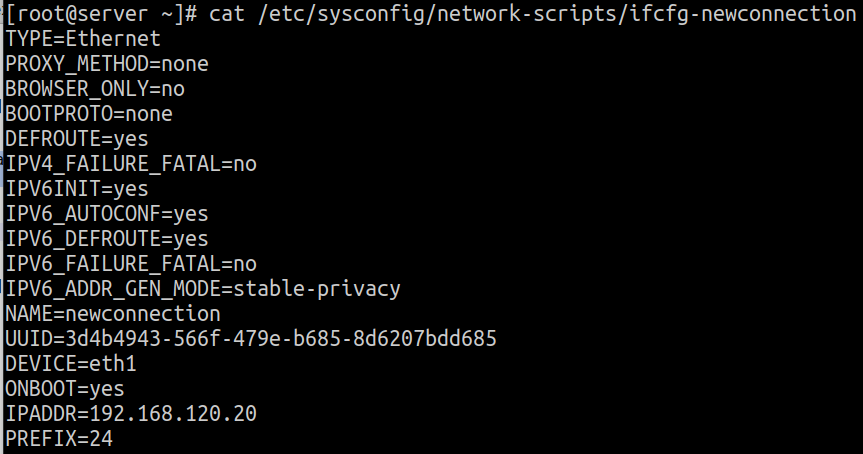
\includegraphics[scale=.35]{content/chapter14/images/networkscript.png}
			\caption{Sample output}
			\label{fig:sample}
		\end{figure}		
	
		\bigskip
		\bigskip
	
		\item Command to set gateway \& dns:
		\begin{tcolorbox}[breakable,notitle,boxrule=-0pt,colback=pink,colframe=pink]
			\color{black}
			\fontdimen2\font=1em
			Syntax: nmcli connection modify <connection\_name> ipv4.gateway <ip\_address> ipv4.dns <ip\_address>
			\fontdimen2\font=4pt
		\end{tcolorbox}
		Eg:	
		\begin{tcolorbox}[breakable,notitle,boxrule=-0pt,colback=black,colframe=black]
			\color{green}
			\fontdimen2\font=1em
			\# nmcli connection modify newconnection ipv4.gateway 192.168.122.1 ipv4.dns 192.168.122.254
			\fontdimen2\font=4pt
		\end{tcolorbox}
	
		
			
	
	
	\end{itemize}
	
	
\end{itemize}



\end{flushleft}
\newpage


